\section{全幺模性}
\label{sec:graph-incidence-total-unimodularity}
\label{sec:incidence-tu-definition}

前面两节建立了顶点函数和边函数的空间，并给出了正交分解和维数。现在转向另一个问题：如果把图上的流量或选边写成线性规划，什么时候即使放开整数约束，最优解仍然是整数？答案取决于系数矩阵的方子式——这就是全幺模性。

举一个小例子。矩阵
\[
\bm{M}=\begin{pmatrix}1&1\\1&-1\end{pmatrix}
\]
的每个条目都是$\pm1$，但$\det\bm{M}=1\cdot(-1)-1\cdot1=-2$。以$(1,0)^\top$为右端解方程$\bm{M}\bm{x}=(1,0)^\top$，克莱姆法则给出
\[
x_1=\frac{\det\begin{pmatrix}1&1\\0&-1\end{pmatrix}}{\det\bm{M}}=\frac{-1}{-2}=\frac{1}{2},\qquad
x_2=\frac{\det\begin{pmatrix}1&1\\1&0\end{pmatrix}}{\det\bm{M}}=\frac{-1}{-2}=\frac{1}{2}.
\]
分母$-2$正是行列式的值。只要行列式不是$\pm1$，这种除法就可能产生分数。

全幺模性从根本上排除这个问题：它要求从矩阵中取出任意方形子矩阵时，所得行列式都属于$\{0,1,-1\}$。

\begin{definition}[全幺模矩阵]
\label{def:graph-total-unimodularity}
若矩阵的每个方形子矩阵的行列式都属于$\{0,1,-1\}$，就称它为\term{全幺模矩阵}（totally unimodular matrix，简称TUM）。
\end{definition}

取一阶方子式就是单个条目，因此全幺模矩阵的每个元素只能是$0$、$1$或$-1$。但上面的$\bm{M}$说明，仅检查条目远远不够——还必须检查所有更高阶的方子式。

\subsection{带符号关联矩阵的全幺模性}
\label{sec:incidence-signed-tu}

前一节定义的关联矩阵$\bm{B}$，每一列在尾端取$+1$、头端取$-1$，其余为零。这种矩阵称为\term{带符号关联矩阵}（signed incidence matrix）。无向图只需为每条边选一个记录方向；反转一条边只让相应列变号，而列变号不改变任何方子式的绝对值，所以全幺模性与方向选择无关。

\begin{theorem}[带符号关联矩阵]
\label{thm:graph-signed-incidence-tu}
有限无自环图的带符号关联矩阵是全幺模矩阵。
\end{theorem}

\begin{proof}
对方子式的阶数$k$做归纳。

$k=1$时，条目本身属于$\{0,1,-1\}$，满足条件。

设所有低于$k$阶的方子式已满足结论，考察$\bm{B}$中任意$k$行$k$列组成的方阵。按这个方阵中各列的结构，分三种情形讨论。

情形一：有一列在方阵中没有保留任何端点行。这一列全为零，含有零列的方阵行列式为零。

情形二：有一列只保留了一个端点行。这一列中唯一的非零元为$+1$或$-1$。沿这一列展开行列式，得到这个$\pm1$乘以一个$(k-1)$阶的余子式。由归纳假设，余子式属于$\{0,1,-1\}$，两者相乘仍属于$\{0,1,-1\}$。

情形三：每一列的两个端点行都保留了下来。此时每列恰有一个$+1$和一个$-1$，列和为零。把方阵的所有行相加，得到零行向量。行向量线性相关意味着行列式为零。

三种情形涵盖了所有可能的列结构，归纳完毕。
\end{proof}

用一个具体的例子来看证明是怎样起作用的。以无向三角形为例，按$1\to2$、$2\to3$、$3\to1$记录方向，关联矩阵为
\[
\bm{B}_\triangle=
\begin{pmatrix}
1&0&-1\\
-1&1&0\\
0&-1&1
\end{pmatrix}.
\]
三行之和为零向量，因此整体行列式为零——这正是情形三。再看左上角的$2\times2$子矩阵$\bigl(\begin{smallmatrix}1&0\\-1&1\end{smallmatrix}\bigr)$：其中第一列只保留了一个端点行（情形二），沿该列展开得到行列式$1$。

注意三角形含有奇数长的环，但这并不影响带符号关联矩阵的全幺模性。证明中用到的只是"每列有一个$+1$和一个$-1$"这个结构性质，与环的奇偶无关。

从$\bm{B}$中删掉若干行后，剩余矩阵的每个方子式仍然是原矩阵的某个方子式。因此约化后的矩阵也全幺模——后面讨论线性规划时删去冗余守恒式会用到这一点。

\subsection{无符号关联矩阵的全幺模性}
\label{sec:incidence-unsigned-tu}

如果只想记录一条边接在哪两个顶点，不需要区分出入方向，就在两个端点对应的行各填一个$1$，其余行填零。按这个规则得到的矩阵$\bm{N}$称为\term{无符号关联矩阵}（unsigned incidence matrix）。

仍用三角形，边序不变。无符号关联矩阵为
\[
\bm{N}_\triangle=
\begin{pmatrix}
1&0&1\\
1&1&0\\
0&1&1
\end{pmatrix}.
\]
与带符号版本的唯一区别是第三列第一行从$-1$变成了$+1$。计算行列式：沿第一行展开，
\[
\det\bm{N}_\triangle=1\cdot(1\cdot1-0\cdot1)-0+1\cdot(1\cdot1-1\cdot0)=1+1=2.
\]
同一张图在两种端点符号约定下产生了不同的行列式值。

\begin{theorem}[无符号关联矩阵]
\label{thm:graph-unsigned-incidence-tu}
有限简单无向图的无符号关联矩阵全幺模，当且仅当该图是二部图。
\end{theorem}

\begin{proof}
先证充分性。若图是二部图，顶点分为两侧$U$和$W$，每条边都连接两侧。把$W$侧对应的所有行乘以$-1$。每一列原先在两个端点都是$+1$，变号后$U$侧的端点留下$+1$，$W$侧的端点变成$-1$。这恰好是把所有边统一从$U$指向$W$得到的带符号关联矩阵。行变号不改变方子式的绝对值（每变号一行使行列式乘$-1$，多行变号的效果相乘）。因此由定理~\ref{thm:graph-signed-incidence-tu}可知原矩阵也全幺模。

再证必要性。若图不是二部图，则存在奇数长度的环。设这个环按顶点$1,2,\ldots,\ell$的次序闭合，$\ell$为奇数。只选这$\ell$个顶点的行和环上$\ell$条边的列（即边$\{1,2\},\{2,3\},\ldots,\{\ell,1\}$），得到一个$\ell\times\ell$方阵。

对这个方阵的行列式作排列展开。每列对应环上的一条边，恰好在两行上有$1$，因此每列必须从两个端点中选一行。选中的行不能重复。

从第一列开始：如果选尾端（行$1$），那么第二列的尾端行$2$还可用，但最后一列$\{\ell,1\}$的行$1$已经被第一列占走，所以最后一列只能选行$\ell$。沿环逐列推导，发现所有列都选尾端。如果第一列选头端（行$2$），那么第二列的行$2$被占，只能选行$3$，继续推理的效果是所有列都选头端。

因此非零排列项恰有两项：恒等排列（每列选尾端）和长度为$\ell$的循环置换（每列选头端）。恒等排列的符号为$+1$。循环置换可以拆成$\ell-1$次对换，而$\ell$为奇数时$\ell-1$为偶数，符号也是$+1$。两项同号，行列式为$1+1=2$，绝对值不属于$\{0,1,-1\}$，因此无符号关联矩阵不全幺模。
\end{proof}

图~\ref{fig:incidence-bipartite-signs}比较了两种环上的符号分配。观察四边环：从顶点$1$开始，沿边依次给下一个顶点分配相反的符号。$\{1,3\}$与$\{2,4\}$分成两侧，把$2,4$对应的行变号后，每条边恰好有一个正端点和一个负端点。再观察三角形：$1$与$2$需异号，$2$与$3$需异号，因此$1$和$3$已被定为同号。但最后一条边$\{3,1\}$连接两个同号端点，无法通过行变号变成一正一负。行列式计算中的$1+1=2$，正是这个符号冲突的具体表现。

\begin{BookInlineFigure}
  \centering
  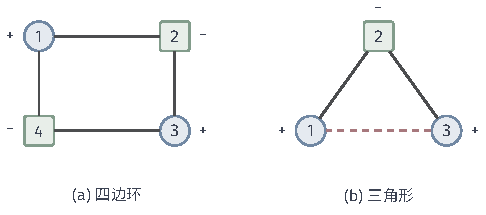
\includegraphics{figures/03-graphs/05-matrices-and-spectra/tikz/incidence-bipartite-signs/figure.pdf}
  \caption{沿环交替分配行符号。圆形顶点保留原行，方形顶点对应的行变号。四边环的每条边都连接异号端点，三角形的虚线边连接两个同号端点。}
  \label{fig:incidence-bipartite-signs}
\end{BookInlineFigure}

\subsection{整数最优解的存在}
\label{sec:incidence-integral-optima}

求最大流时，我们在每个顶点核对流入和流出。求匹配时，在每个顶点数一数选中了几条边。两类问题都是给每条边设一个变量，再用关联矩阵把变量汇总到顶点。如果允许变量取分数值，问题就变成一个普通的线性规划。什么条件能保证放宽后的问题仍有一个整数最优方案？

\subsubsection{关联约束的线性规划}
\label{sec:incidence-lp-models}

把边变量排成向量$\bm{x}$。等式可以规定每个顶点的净流出量，不等式可以限制每条边的容量或每个顶点选边的总量。将等式系数记为$\bm{P}$，上界约束的系数记为$\bm{Q}$，线性松弛可以写成
\begin{equation}
\begin{aligned}
\max_{\bm{x}}\quad &\bm{c}^\top\bm{x}\\
\text{满足}\quad &\bm{P}\bm{x}=\bm{b},\quad
\bm{Q}\bm{x}\leq\bm{d},\quad \bm{x}\geq\bm{0}.
\end{aligned}
\label{eq:incidence-lp-relaxation}
\end{equation}
这里$\bm{b}$和$\bm{d}$是整数数据，$\bm{c}$是目标系数。整数性成立的条件是：把$\bm{P}$和$\bm{Q}$纵向叠在一起得到的矩阵全幺模，并且两个右端都是整数向量。

对每条上界约束，引入一个\term{松弛变量}，记录它还剩多少余量：$\bm{z}=\bm{d}-\bm{Q}\bm{x}\geq\bm{0}$。原来的不等式就等价于$\bm{Q}\bm{x}+\bm{z}=\bm{d}$。把两组等式合在一起，标准型的约束变为
\begin{equation}
\begin{pmatrix}
\bm{P}&\bm{0}\\
\bm{Q}&\bm{I}
\end{pmatrix}
\begin{pmatrix}\bm{x}\\\bm{z}\end{pmatrix}
=
\begin{pmatrix}\bm{b}\\\bm{d}\end{pmatrix},
\qquad \bm{x},\bm{z}\geq\bm{0}.
\label{eq:incidence-lp-slack-matrix}
\end{equation}
每个$\bm{x}$唯一确定一组$\bm{z}$，目标仍为$\bm{c}^\top\bm{x}$。

标准型的系数矩阵右侧多了一个单位阵。看它的任意方子式：如果选中了某个松弛变量的列，这一列在方阵里要么全为零（行列式为零），要么只有一个$1$（沿之展开，阶数降低一）。把选中的松弛列逐一消去，最后剩下的是$\bm{P}$和$\bm{Q}$叠成的矩阵中的一个方子式。如果所有列都是松弛列，消去后空矩阵的行列式按约定等于$1$。因此标准型系数矩阵仍全幺模，右端也仍是整数。

\subsubsection{整数顶点定理}
\label{sec:incidence-integral-vertex-theorem}

把式~\eqref{eq:incidence-lp-slack-matrix}中的原变量和松弛变量合在一起记为$\bm{y}$，右端记为$\bm{r}$，目标系数记为$\bm{a}$（松弛变量的目标系数为零）。标准型变成
\begin{equation}
\max_{\bm{y}}\ \bm{a}^\top\bm{y}
\qquad
\text{满足}\quad \bm{A}\bm{y}=\bm{r},\quad \bm{y}\geq\bm{0}.
\label{eq:incidence-lp-standard}
\end{equation}
线性规划可行且最优值有限时，顶点定理保证最优值能在可行域的某个顶点取得。这里的"顶点"是指不能写成两个不同可行点的凸组合的点。要保证整数最优解存在，只需证明每个顶点的坐标都是整数。顶点定理可参考\BookChapterRef{chap:linear-programming}{卷五"线性规划"章}。

\begin{theorem}[标准型的整数顶点]
\label{thm:graph-tu-integral-vertices}
设式~\eqref{eq:incidence-lp-standard}的系数矩阵$\bm{A}$全幺模，右端$\bm{r}$为整数向量。则可行域的每个顶点都是整数向量。若问题可行且最优值有限，则至少存在一个整数最优解。
\end{theorem}

\begin{proof}
可行域为空时没有顶点需要考察。以下设可行域非空，记$r=\operatorname{rank}\bm{A}$。

先做约化。从$\bm{A}$中选取$r$个线性无关的行，保留对应的右端分量。被删的每一行是所选行的线性组合，把任意可行点代入，可知被删行的右端也是所选右端分量的同一线性组合——因此保留的等式已能推出全部等式。约化后的系数矩阵仍全幺模（方子式只会减少），右端仍为整数。以下继续用$\bm{A}$和$\bm{r}$表示约化后的数据。

若$r=0$，等式约束为空，可行域是$\{\bm{y}\geq\bm{0}\}$。其中每个非零可行点至少有一个正坐标$y_j>0$，沿第$j$个方向正反各动一小步就能把它写成两个不同可行点的中点，所以它不是顶点。只有零向量可能是顶点，它当然是整数向量。以下设$r>0$。

取任意顶点$\bm{y}^\star$，记$S=\{j:y_j^\star>0\}$为正坐标的下标集。我们分三步说明$\bm{y}^\star$为何是整数向量。

第一步：$S$对应的列线性无关。如果相关，就存在非零向量$\bm{h}$，在$S$之外全为零且$\bm{A}\bm{h}=\bm{0}$。取充分小的$\varepsilon>0$使得$\bm{y}^\star\pm\varepsilon\bm{h}$的$S$内坐标仍正，$S$外坐标仍为零。这两个不同的可行点以$\bm{y}^\star$为中点，与顶点定义矛盾。

第二步：将$S$的列补成一组基。$S$对应的独立列数$|S|\leq r$，补选一些列使下标集扩充为$r$列的$J$，令$\bm{A}_J$可逆。$J\setminus S$中的坐标及$J$之外的坐标全为零，因此
\[
\bm{A}_J\bm{y}^\star_J=\bm{r},\qquad \bm{y}^\star_{J^c}=\bm{0}.
\]
$\bm{A}_J$称为\term{基矩阵}，$\bm{y}^\star$是这组基给出的\term{基本可行解}。

第三步：用克莱姆法则求解。$\bm{A}_J$是全幺模矩阵的可逆方形子矩阵，行列式只能为$\pm1$。令$\bm{A}_J^{(i)}$为将$\bm{A}_J$的第$i$列换成$\bm{r}$后的矩阵，克莱姆法则给出
\[
(\bm{y}^\star_J)_i=\frac{\det(\bm{A}_J^{(i)})}{\det(\bm{A}_J)}.
\]
分子是整数矩阵的行列式，本身为整数。分母为$\pm1$。因此每个基坐标都是整数。非基坐标全为零，也是整数。

最后，可行且最优值有限时，由顶点定理取一个最优顶点，它已被证明为整数向量。
\end{proof}

从基矩阵的逆也能看到整数性。由求逆公式，
\[
\bm{A}_J^{-1}=\frac{\operatorname{adj}(\bm{A}_J)}{\det(\bm{A}_J)}.
\]
伴随矩阵$\operatorname{adj}(\bm{A}_J)$的每个条目是一个低一阶的方子式乘以符号，全幺模性保证它们属于$\{0,1,-1\}$。分母为$\pm1$，所以$\bm{A}_J^{-1}$是整数矩阵。用它乘整数右端$\bm{r}$，自然得到整数基坐标。

\subsubsection{图上的整数解}
\label{sec:incidence-integrality-applications}

回到图上的两类问题，分别检查它们的系数矩阵是否满足全幺模条件。

在流量问题里，每个顶点的守恒等式由带符号关联矩阵$\bm{B}$给出，每条弧的容量上界由单位行给出。把$\bm{B}$和$\bm{I}$纵向叠在一起后，任意方子式要么完全来自$\bm{B}$的行列，要么通过沿单位行展开后降阶仍落到$\bm{B}$的子式中。因此堆叠后的矩阵仍全幺模。

在二部匹配问题里，每个顶点的选边额度由无符号关联矩阵$\bm{N}$给出约束$\bm{N}\bm{x}\leq\bm{1}$。每条边恰好连接两个受限的顶点，所以每个$x_e$都被约束在$[0,1]$内。二部图的$\bm{N}$本身已经全幺模（定理~\ref{thm:graph-unsigned-incidence-tu}），松弛变量的单位列不改变全幺模性。

两类问题的右端都是整数，变量都有上界使可行域有界。定理~\ref{thm:graph-tu-integral-vertices}保证只要问题可行，就存在整数最优解。对匹配来说，整数边变量只能取$0$或$1$：$1$表示选中这条边，$0$表示不选。

最大流的流值$F$本身也是变量。图~\ref{fig:incidence-flow-integer-example}展示了一种处理方式：添加一条回流弧$t\to s$，使回流弧的流量$q_4$等于原网络的流值。加上回流弧后，每个顶点（包括源和汇）的守恒式都取零右端。目标就是最大化回流弧上的流量。删去回流弧就还原原图中的流。图中的三点网络里，中转路线$s\to a\to t$受容量$1$限制，直达路线$s\to t$的容量也是$1$，两条各运一个单位，达到最大流值$2$。如果是给定整数供需的最小费用流，则直接以指定的净流出量作为右端。

\begin{BookInlineFigure}
\centering
\begin{tikzpicture}[
  x=1.16cm, y=1cm,
  point/.style={circle,draw=incFlowBlue,fill=incFlowLight,
    minimum size=6mm,inner sep=0pt,line width=.75pt},
  arc/.style={-{Stealth[length=2.2mm]},draw=incFlowLine,line width=.85pt}
]
\definecolor{incFlowBlue}{HTML}{7188A3}
\definecolor{incFlowLight}{HTML}{E5EAF0}
\definecolor{incFlowLine}{HTML}{4C4D4F}
\definecolor{incFlowGreen}{HTML}{829C8B}
\node[point] (s) at (0,0) {$s$};
\node[point] (a) at (2,1.13) {$a$};
\node[point] (t) at (4,0) {$t$};
\draw[arc] (s) -- node[above left] {$q_1\;(2)$} (a);
\draw[arc] (a) -- node[above right] {$q_2\;(1)$} (t);
\draw[arc] (s) -- node[above] {$q_3\;(1)$} (t);
\draw[arc,draw=incFlowGreen,dashed] (t) to[bend left=26]
  node[below] {$q_4\;(3)$} (s);
\end{tikzpicture}

\caption{三点最大流网络。实线标出三条原有弧，括号内是容量。虚线是为守恒记账加上的回流弧，其流量$q_4$等于原网络的流值。}
\label{fig:incidence-flow-integer-example}
\end{BookInlineFigure}

图~\ref{fig:incidence-matching-comparison}对照了全幺模条件成立和失效时的选边方案。

在四边环上，两个交替选边的整数方案各选两条不相邻的边，总量为$2$。四条边各取$1/2$是这两个方案的平均，也达到最优值$2$。这说明整数最优解与分数最优点可以并存。

在三角形上，每条边取$1/2$恰好用满三个顶点的额度，总量为$3/2$。把三个约束$x_{12}+x_{23}\leq1$、$x_{12}+x_{13}\leq1$、$x_{23}+x_{13}\leq1$相加并除以$2$，可知$3/2$已经是松弛问题的上界。而整数匹配最多选一条边，最优值只有$1$。这个间隙的来源正是三角形的无符号关联矩阵行列式为$2$——克莱姆法则中的除法产生了$1/2$。

\begin{BookInlineFigure}
  \centering
  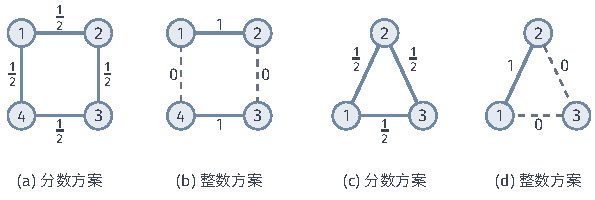
\includegraphics{figures/03-graphs/05-matrices-and-spectra/tikz/incidence-matching-comparison/figure.pdf}
  \caption{四边环和三角形上的选边方案。每个顶点周围的选边量之和都不超过$1$。边旁的数是选边量，实线表示该量为正，虚线表示为零。(a)、(b) 的总量均为$2$，(c)、(d) 分别为$3/2$和$1$。}
  \label{fig:incidence-matching-comparison}
\end{BookInlineFigure}

具体的求解方法见第~\ref{chap:max-flow-min-cut}章、第~\ref{chap:min-cost-flow}章和第~\ref{chap:bipartite-matching-assignment}章。